\documentclass[conference, a4paper]{IEEEtran}
%\IEEEoverridecommandlockouts
% The preceding line is only needed to identify funding in the first footnote. If that is unneeded, please comment it out.
\usepackage{cite}
\usepackage{amsmath,amssymb,amsfonts}
\usepackage{algorithmic}
\usepackage{graphicx}
\graphicspath{{images/}}
\usepackage{textcomp}
\usepackage{xcolor}
\usepackage{hyperref}
\usepackage{fancyhdr}
\usepackage{filecontents}
\usepackage{graphicx}
\renewcommand{\headrulewidth}{0pt}
\pagestyle{fancy}
\lfoot{Methods for Detecting Denial-of-Service Attacks}
\cfoot{}
\rfoot{\thepage}
\usepackage[belowskip=-15pt,aboveskip=0pt]{caption}
\hypersetup{
    colorlinks=false,
    pdfborder={0 0 0},
}

\def\BibTeX{{\rm B\kern-.05em{\sc i\kern-.025em b}\kern-.08em
    T\kern-.1667em\lower.7ex\hbox{E}\kern-.125emX}}
\begin{document}

\title{Methods for Detecting Denial-of-Service Attacks\\
}

\author{\IEEEauthorblockN{Owen Prosser}
\IEEEauthorblockA{\textit{School of Computer Science} \\
\textit{University of Lincoln}\\
Lincoln, United Kingdom \\
14514822@students.lincoln.ac.uk}
}

\maketitle

\begin{abstract}
    Lorem ipsum dolor sit amet, consectetur adipiscing elit. Pellentesque aliquam orci eget tellus luctus mollis. Aliquam erat volutpat. Praesent malesuada, sapien quis vestibulum porta, felis augue vehicula massa, non laoreet turpis purus eget nunc. Phasellus faucibus metus nunc, in lacinia massa hendrerit nec. In tempus luctus justo, in placerat ex posuere sed. Vivamus convallis vitae velit quis dignissim. Phasellus placerat, ex non tempor ultricies, lacus est scelerisque augue, non commodo odio nisl in ante. Nam turpis nisl, efficitur eu rutrum at, porta vel quam. Vestibulum eget elit malesuada, feugiat ex sed, finibus nunc. Aliquam nec eros ex. Duis ut lectus.
    \newline
\end{abstract}

\begin{IEEEkeywords}
    Denial of Service, DoS, Cyber Security
\end{IEEEkeywords}

    Information Security and Network Resilience has become increasingly important as society has become reliant on technology to function.
    Over the last 20 years Denial of Service attacks (Dos) have become more disruptive. The volume of attacks has increased, the distribution across the globe has become greater and they have been easier to launch \cite{20_years_of_DDOS}.
    One example of this is the effect that cyber attacks can have on infrastructure such as Power Systems \cite{DDOS_power_systems}. 
    This in conjunction with the rise in popularity of the devices considered to be a part of the Internet of Things (IoT), has lead to an increase in the ability of malicious actors to launch large scale attacks.

    Whilst this kind of attack does not come with any risk to sensitive data which may be held on the targeted machines, it is still considered to be very disruptive.
    In 2019 7\% of Businesses reported that the Denial-of-Service attacks were the most disruptive Cyber attack that they have fallen victim to in the last 12 months.
    This percentage is even higher (14\%) among Information and Communications firms.\cite{government_security_survey}

    One way which networks can be disrupted is a technique known as a Denial of Service attack (DoS).
    Such an attack works by consuming the resources of a computer or a network of computers so that they cannot effectively perform their intended task.
    In addition to Denial of Service attacks there are also a similar attack called a Distributed Denial of Service attack (DDoS).
    The first of these attacks occurred in 1999 when a botnet called 'Trin00' took down a network at the University of Minnesota. \cite{CERT_DDOS}

\section{Types of Attacks}
\subsection{Denial of Service}
\subsection{Distributed Denial of Service}
    A Distributed Denial of Service attack (DDoS) is similar to a more rudimentary DoS attack and generally separated into two categories; Direct and Reflector attacks.

    In a Direct attack, the attacker will flood the target host or server with a vast amount of packets from a large number of compromised hosts or machines.
    A Direct attack can then also be segmented into two more categories. There are Network Layer DDoS attacks and Applications Layer DDoS attacks.\cite{empirical_evaluation}

    An Application layer DDoS attack is one which specifically attacks the top the layer of the OSI model, the application layer.
    These type of attacks exploit the amount of processing power used by common protocols such as HTTP/POST and HTTP/GET.
    They can cause a high computational load on the target machines without being required to send large amounts of data as each request can require a lot a processing time on the targets hardware.
    Using such a method an attacker can still have a large disruptive effect, without them needing to use as much bandwidth.\cite{cloudflare_DDoS}

    A network layer DDoS attack is designed to take a target computer offline by consuming all of the available network resources so that the target cannot respond to legitimate requests.
    One example of this is SYN flooding, the most common DDoS attack technique. \cite{chnage_point_monitoring} Using this attack, an attacker would overwhelm a target machine by repeatedly sending initial connection request (SYN) packets.
    Each of these packets would have a spoofed IP address so that when the target sends the syn-acknowledgement packet it is keeping a port open, waiting for a response which will never come.
    Once all of the ports of the machine are open and waiting for responses, the machine will not be able to respond to legitimate requests.\cite{cloudflare_syn_flood}

\subsection{Low-Rate Denial of Service}
    Low-rate attack traffic is generally similar to legitimate traffic; making it difficult to identify distinguish.\cite{two_layer_approach__DDOS}
    This is because it uses a small amount of bandwidth to keep open a port on the target machine for as long as possible.
    One method of archiving this is to send partial HTTP headers, the target machine will then keep the connection open waiting for the rest of the data to arrive.
    Like the syn-flooding method this will also prevent the target from responding to legitimate traffic once all of the ports are occupied waiting for responses.
    This can be a difficult attack to mitigate against as these type of intensionally slow connections are difficult to distinguish from actual users on legitimately slow connections because the traffic is very similar.\cite{cloudflare_low_rate}

\section{Detection Methods}
    Detecting DoS attacks can be challenging as many techniques "face the considerable challenge of discriminating network-based flooding attacks from sudden increases in legitimate activity or flash events".\cite{detection_methods_2006}
    Failing to discriminate between traffic could cause a network to go offline unnecessarily.

    Most DoS protection systems are broken up into two main categories, Signature-based and Anomaly-based systems.
    Signature-based systems inspect passing traffic and searches for already-known malicious patterns.
    On the other hand an anomaly-based system will observe the usual patterns of network traffic and then trigger when it notices a pattern of traffic deemed to be out of the ordinary.
    Most DoS prevention systems are anomaly based.\cite{chnage_point_monitoring}

    \subsection{Anomaly Detection}
        An anomaly is described as  "an observation which deviates so much from other observations as to arouse suspicions that it was generated by a different mechanism". \cite{hawkins_quote}
        An anomaly is treated as an important event because anomalous activity or traffic can be a good indication of something malicious. 
        Figure \ref{fig:anomaly_overview} shows a generic overview of how an anomaly detection system would operate.
        This diagram can make such a system seen straight-forward to implement but there are many factors which complicate such a solution.
        Some of these factors are detailed below: \\
            \begin{itemize}
                \item There is no detection method which would be applicable to all situations. For example an monitoring system for a wired local network could be different to a wireless local network.
                \item The data which is being monitored would likely contain noise which could be difficult to filter out or could lead to false positives.
                \item There is no universally available datasets which could be used to train a classifier to monitor a system. Gathering a dataset could be time consuming, expensive or impossible.
                \item 'Normal' behaviors are often changing which could result in a system needing constant maintenance or else be prone to errors.\\
            \end{itemize}
        With the ever-increasing rate-of-change of technology and use of the internet, anomaly detection has become more challenging to implement than ever.
        It also has the significant issue, due to its training coming from previously recorded data, it is unable to detect zero-day vulnerabilities.\cite{anomaly_survey}
        
        \subsubsection{Change-Point Monitoring}
            Like any anomaly-based monitoring systems a Change-Point Monitoring (CPM) system compared currently observable sequence with historical data to detect anomalies.
            The difference with the type of system however, is that a CPM is monitoring the network traffic protocol behaviors rather than a users traffic patterns. 
            "For instance, according to the specification of TCP/IP protocol, in its normal operation, a FIN (RST) is paired with a SYN at the end of data transmission".
            A CPM system tracks how network traffic follows the specification of its respective protocol and an influx of discrepancies could be considered an event. \cite{CPM}

        The difficulties in implementing, and gathering the required dataset for, a anomaly detection system limit its applicability to this project.
        Due to the inherent time constants of a Masters Dissertation, much of the available time would be consumed gathering the dataset as it is unlikely that a suitable, openly-available, one could be found.

        \begin{figure}
            \centering
            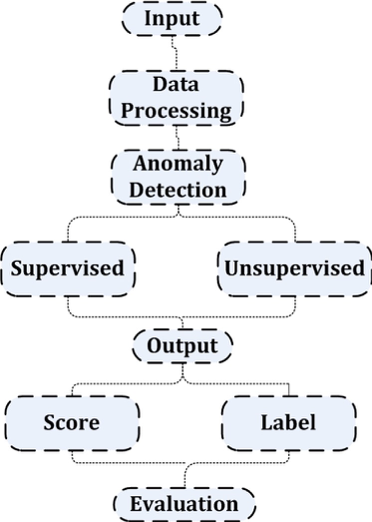
\includegraphics[width=5cm]{images/anomaly_diagram.png}
            \caption{Overview of Anomaly Detection system \cite{anomaly_survey}}
            \label{fig:anomaly_overview}
        \end{figure}

    \subsection{Low-rate Denial of Service Attack Detection}
        Low-rate attacks are more difficult to detect than standard denial of service attacks; their behavior is more similar to the standard behavior of a legitimate user than a flooding attack.
        This makes them more likely to produce false positives if not effectively implemented when compared to other anomaly detecting methods. 
        

\section{Conclusions}
    The main factors limiting the scope of this project is the available time.
    With less than three months to research, design, implement and test a system. Any tasks which can be time-expensive, such a gathering a dataset, need to limited as much as possible.
    This limitation lends the project more towards a detection method which is based on lower-level traffic analysis, looking for discrepancies in the structure of the network traffic.
    This approach would also mitigate another limiting factor, the hardware resources available. For a project such as this having any kind of large network or computer system for development and testing is impossible.
    The project is going to need to be designed to be built, and operated, on a much smaller scale then the methods discussed in this review.
    This will result in a small amount of network traffic being monitored by the potential system, allowing for more time for analysis of each packet.

\begin{thebibliography}{00}
    \bibitem{20_years_of_DDOS}Osterweil, E., Stavrou, A. and Zhang, L., 2019. 20 Years of DDoS: a Call to Action. arXiv preprint arXiv:1904.02739.
    \bibitem{DDOS_power_systems}Chen, W., Ding, D., Dong, H. and Wei, G., 2019. Distributed Resilient Filtering for Power Systems Subject to Denial-of-Service Attacks. IEEE Transactions on Systems, Man, and Cybernetics: Systems.
    \bibitem{government_security_survey}\url{https://www.gov.uk/government/statistics/cyber-security-breaches-survey-2019}
    \bibitem{CERT_DDOS}CERT Coordination Center. 1999. CERT Incident Note IN-99-04. \url{https://web.archive.org/web/20081115163511/http://www.cert.org/incident_notes/IN-99-04.html}Available at \url{https://web.archive.org/web/20081115163511/http://www.cert.org/incident_notes/IN-99-04.html}
    \bibitem{detection_methods_2006}Carl, G., Kesidis, G., Brooks, R.R. and Rai, S., 2006. Denial-of-service attack-detection techniques. IEEE Internet computing, 10(1), pp.82-89.
    \bibitem{nomaly-based_method_for_DDoS}Karimazad, R. and Faraahi, A., 2011, September. An anomaly-based method for DDoS attacks detection using RBF neural networks. In Proceedings of the International Conference on Network and Electronics Engineering (Vol. 11, pp. 44-48).
    \bibitem{empirical_evaluation}Bhuyan, M.H., Bhattacharyya, D.K. and Kalita, J.K., 2015. An empirical evaluation of information metrics for low-rate and high-rate DDoS attack detection. Pattern Recognition Letters, 51, pp.1-7.
    \bibitem{chnage_point_monitoring}H. Wang, D. Zhang, and K. G. Shin, “Change-point monitoring for the detection of DoS attacks,” IEEE Trans. Dependable Secur. Comput., vol. 1, no. 4, pp. 193–208, 2004.
    \bibitem{cloudflare_DDoS}\url{https://www.cloudflare.com/learning/ddos/application-layer-ddos-attack/}
    \bibitem{cloudflare_syn_flood}\url{https://www.cloudflare.com/learning/ddos/syn-flood-ddos-attack/}
    \bibitem{two_layer_approach__DDOS}Toklu, S. and Şimşek, M., 2018. Two-Layer Approach for Mixed High-Rate and Low-Rate Distributed Denial of Service (DDoS) Attack Detection and Filtering. Arabian Journal for Science and Engineering, 43(12), pp.7923-7931.
    \bibitem{cloudflare_low_rate}\url{https://www.cloudflare.com/learning/ddos/ddos-low-and-slow-attack/}
    \bibitem{hawkins_quote}Hawkins D. Identification of outliers (monographs on statistics and applied prob-ability). 1st ed. Netherlands: Springer; 1980.
    \bibitem{anomaly_survey}M. Ahmed, A. Naser Mahmood, and J. Hu, “A survey of network anomaly detection techniques,” J. Netw. Comput. Appl., vol. 60, pp. 19–31, 2016.
    \bibitem{CPM}H. Wang, D. Zhang, and K. G. Shin, “Change-point monitoring for the detection of DoS attacks,” IEEE Trans. Dependable Secur. Comput., vol. 1, no. 4, pp. 193–208, 2004.

\end{thebibliography}

\vspace{12pt}

\end{document}